\documentclass[12pt]{article}

\title{Image Analysis Coursework}
\author{James Hughes\\ Word count: 0}

\usepackage{amsfonts}
\usepackage{amsmath}
\usepackage{graphicx}

\begin{document}

\maketitle

\newpage

\tableofcontents

\newpage

\section{Introduction}

\section{Image Segmentation}

\subsection{CT Image}

\begin{figure}[hp]
    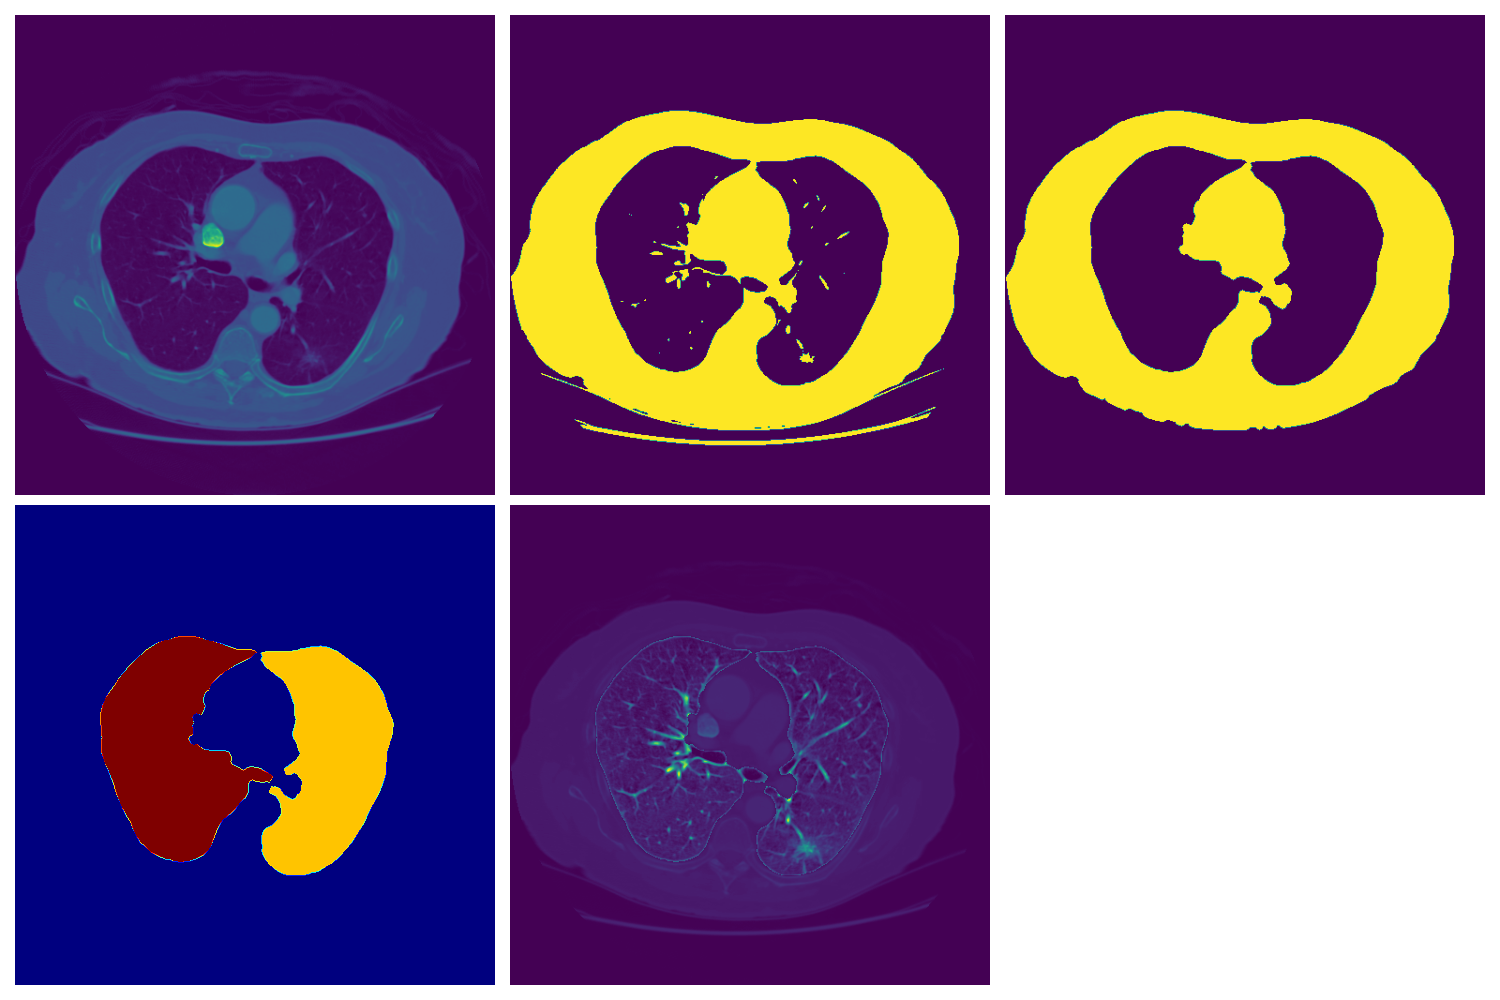
\includegraphics[scale=0.35]{figures/ct_segmentation.png}
    \caption{Steps of CT Segmentation}
    \label{fig:ct}
\end{figure}

The CT scan image was segmented using Otsu's method for image segmentation.
This was an appropriate, simple method which is suited to the monochrome image.
This method easily segments the tissue and bone surrounding the lungs,
distinguishing this from the lugns themselves and the surrounding background.
The segmented image was then post-processed with `binary closing', a morphological operation,
as well as Scikit-Image's \texttt{morphology.remove\_small\_objects} method.
The four segmented regions of the image were then labelled, and the lungs chosen as the smallest masks by area.

\subsection{Flowers Image}

\begin{figure}[hp]
    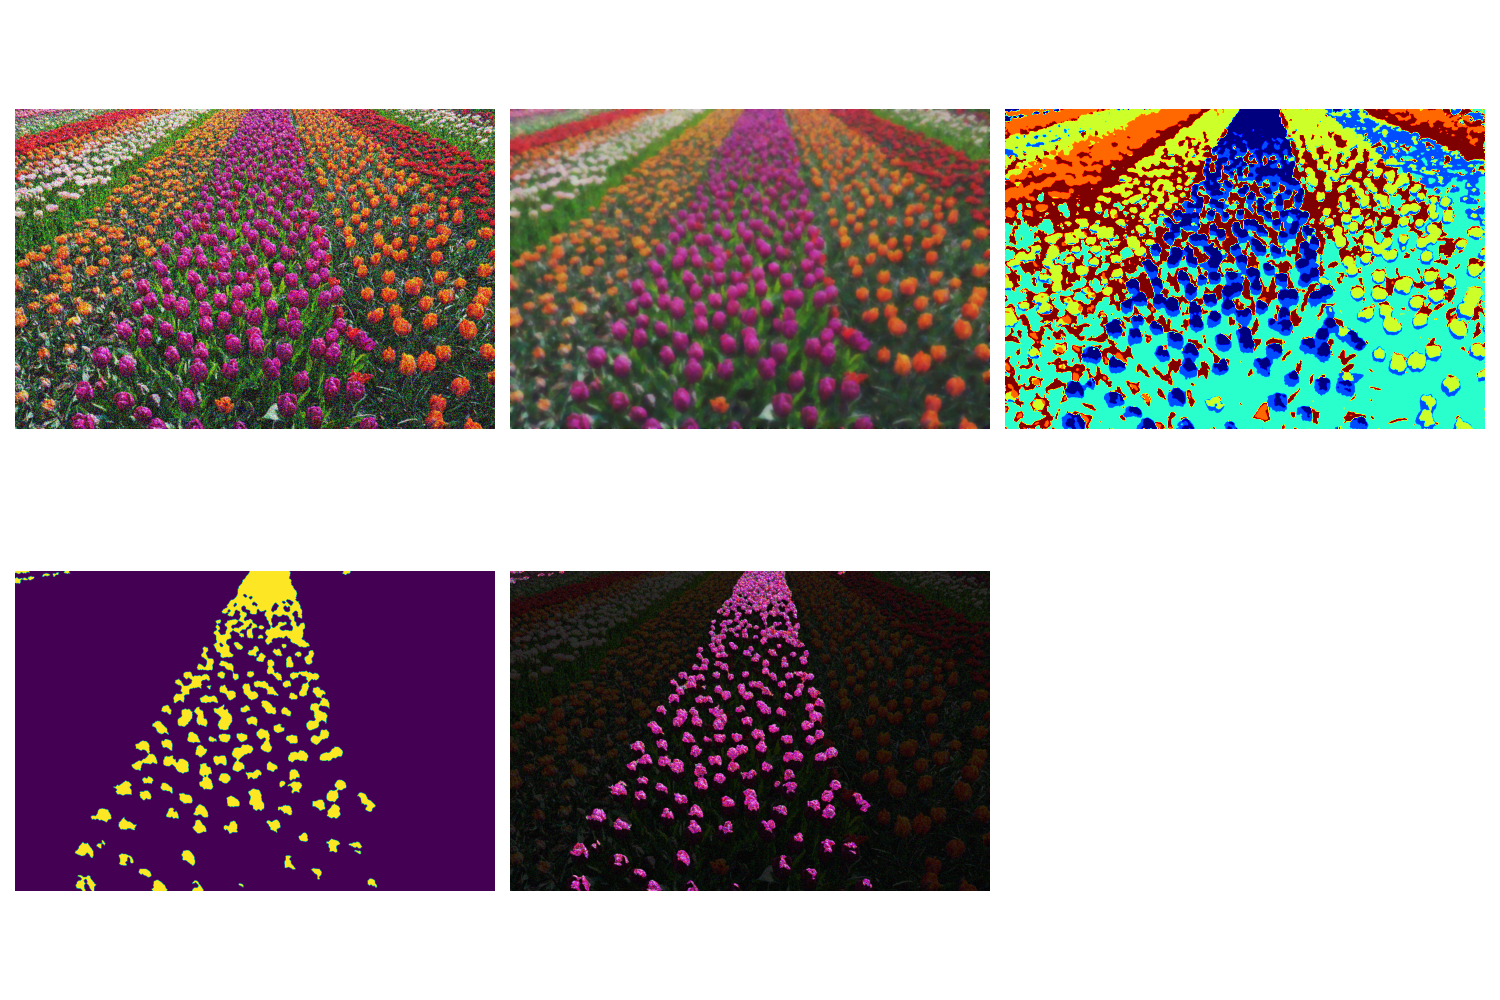
\includegraphics[scale=0.35]{figures/flowers_segmentation.png}
    \caption{Steps of Flowers Segmentation}
    \label{fig:flowers}
\end{figure}

For the flowers image, a more sophisticated segmentation was required in order to handle the three colour channels of the pixels,
as well as to produce a more complex segmentation mask composed of lots of small disconnected regions.
Since the desired segmentation was to be based on the colours present in the image,
it was less important to incorporate local pixel information into the image,
therefore making clustering an appropriate strategy.
In particular, KMeans was chosen, since this method was simple to implement,
commonly used for image segmentation,
and enabled a fixed number of clusters to be specified.
In this case, six clusters was decided as a meaningful number,
corresponding roughly to two shades of green (grass) and four flower colours.
KMeans was implemented as a \texttt{class} in the \texttt{ml} module according to Lloyd's Algorithm \cite{lloyd},
using the kmeans++ \cite{kmeanspp} centroid initialisation method.

Based on this choice of algorithm, Total Variation denoising was used to pre-process the image.
This meant that in the pre-processed image, pixel values were coerced to be similar to those nearby.
This ensured that the clustering algorithm was more stable (since it artificially made the cluster structure of the data more pronounced),
and that the segmentation masks weren't too fine-grained.

The same morphological post-processing from the CT image was used again,
in order to remove segmentation masks that were smaller than the flower buds.

\subsection{Coins Image}

A strong degree of preprocessing was helpful for this image, to assist the segmentation algorithm.
Firstly, the image has been corrupted with vertical columns of pixels that have been masked with zero values.
This was addressed by applying a local median filter.
The locality of this filter was set to each pixel plus its 6 closest horizontal neighbours.
This was wide enough to ensure that in most cases the majority of these 7 pixels are not corrupted,
even in regions where the image is affected more strongly.
An unsharp filter is then used to increase the difference in pixel values within the coin regions compared to just outside of these regions.

To segment all of the coins, the Chan-Vese \cite{chanvese} segmentation algorithm was used.
This method relies on the iterative minimisation of an energy function,
which describes the desired segmentation properties mathematically.
In particular, this technique models the segmentation mask as the set ${x\in\Omega:\phi(x)>0}$,
where $\Omega\subset\mathbb{R}^2$ is the space representing the image,
and $\phi:\Omega\rightarrow[0,1]$ is a function which evolves over the course of the computation.
The function is evolved iteratively to minimise the objective

\begin{align*}
    F(\phi, c_1, c_2) = & \mu\int_{\Omega}\delta(\phi)|\nabla\phi|dxdy + \nu\int_{\Omega}H(\phi)dxdy \\
                    & + \lambda_1\int_{\Omega}|u_0-c_1|^2H(\phi)dxdy + \lambda_2\int_{\Omega}|u_0-c_2|^2(1-H(\phi))dxdy \\
\end{align*}

where $\mu,\nu,\lambda_1,\lambda_2$ are all fixed hyperparameters.
The first two terms serve to regularise the segmentation,
by minimising the length of the segmentation boundary and the segmented area respectively (the area term is ignored in the code).
The second two terms seek to minimise the deviations of pixel values within, and outside, the segmented area from two distinct `representative values',
$c_1$ and $c_2$.
It is worth noting that for any $\phi$, these values minimise the energy when they are the average pixel values in the two corresponding areas of the image.

The algorithm highlighted the background of the image.
Thus to get masks of the coins, the segmentation values were permuted in ${0,1}$ and the segmentation was again post-processed with a morphological closing operation.
The masks were then labelled, and the correct labels were identified via `test pixels', which are seen marking the original image (top-left) in yellow in Figure \ref{fig:coins}

\begin{figure}[hp]
    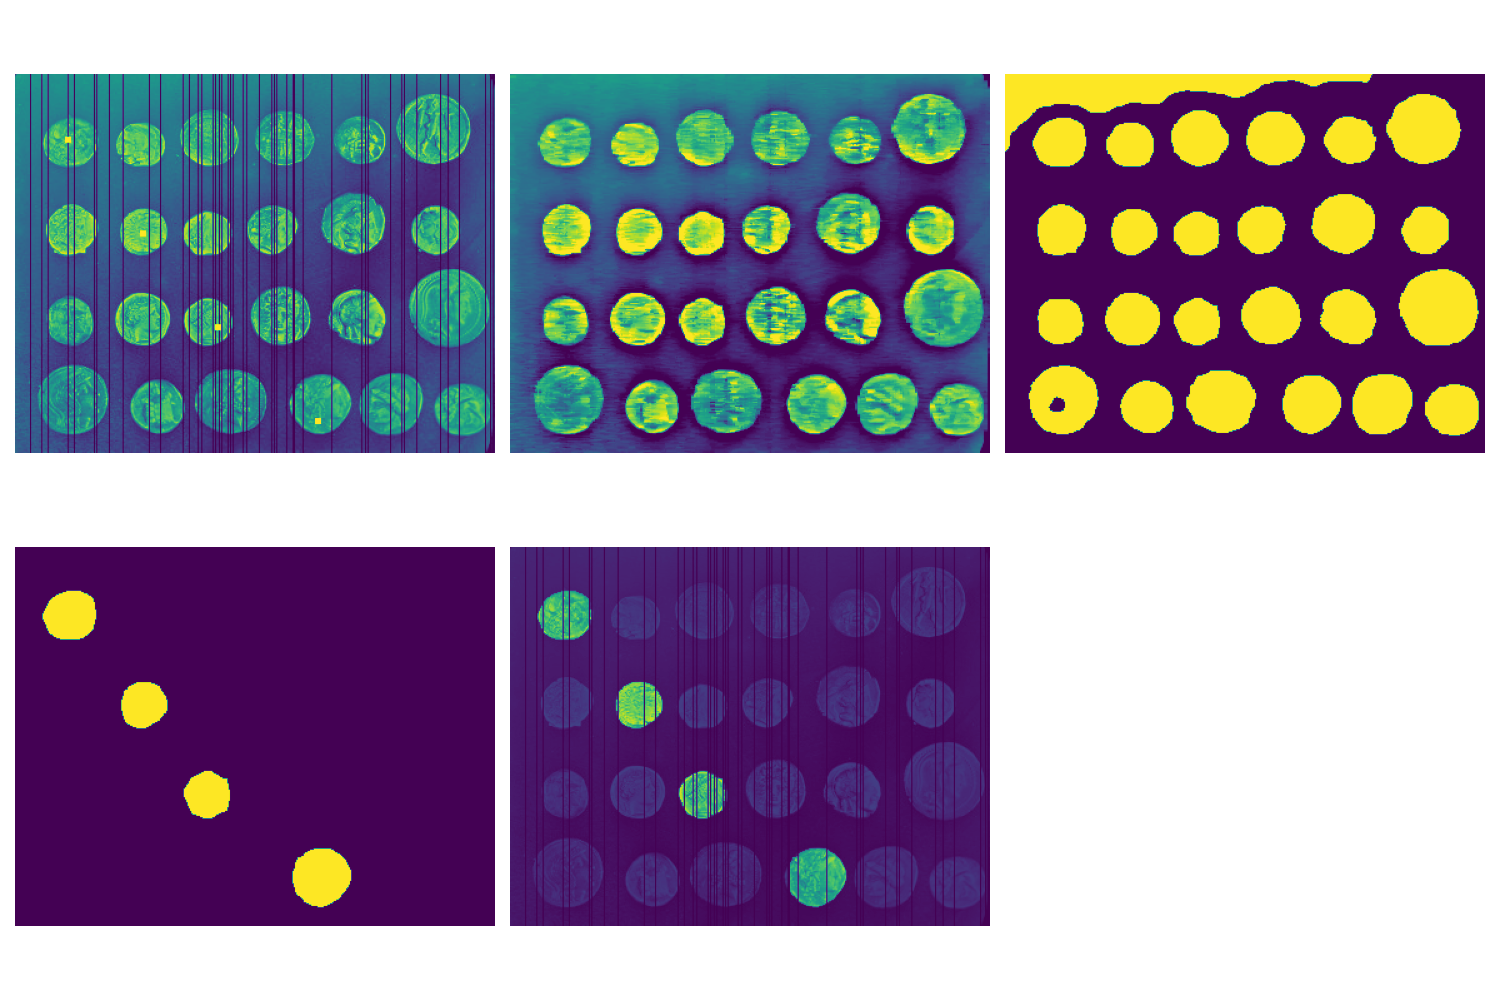
\includegraphics[scale=0.35]{figures/coins_segmentation.png}
    \caption{Steps of Coins Segmentation}
    \label{fig:coins}
\end{figure}

\section{Exploiting Sparsity in Signal Processing}



\section{Algorithms for Solving Inverse Problems}
\subsection{Convergence of Gradient Descent}

Gradient Descent.

We can prove that the given function $f:\mathbb{R}^2\rightarrow\mathbb{R}$ defined

\[f(x_1,x_2) = x_1^2 + \frac{x_2^2}{2}\]

is $L$-smooth with $L=2$ via the following

The result given is, for learning rate $\eta=\frac{1}{L}$, and an $L$-smooth function $f$,

\[f(x_K) - f(x^*) \leq \frac{L||x_0-x^*||_2^2}{2K}\]

It is important to note that this is an estimate that gives the accuracy as $\mathcal{O}(\frac{1}{K})$.
We can use it to compute the estimate the number of steps to required to reach $\epsilon=0.01$,
but this will be an upper bound.
Nonetheless, we can set the right-hand side to $\epsilon$ and rearrange to give:

\[K = \frac{L||x_0-x^*||_2^2}{2\epsilon}\]

Substituting $\epsilon=0.01$, $x^*=(0,0)$, $x_0=(1,1)$, $L=2$, we get $K=200$.

\section{Discussion}
Results/conclusions
Further work
What I learned
How I could have improved \cite{keypaper}

\bibliographystyle{IEEEtran}
\bibliography{Biblio}

\appendix

\section{Statement on the use of auto-generation tools}

\end{document}
